% Slides for 2025-07-01
%To create a slide, use the following:

% To create a slide with a bullet list, use the following:
% \begin{frame}{TITLE}
%     \begin{itemize}
%         \item ITEM 1
%         \item ITEM 2
%     \end{itemize}    
% \end{frame}

% To create a slide with numbered list, use the following:
% \begin{frame}{TITLE}
%     \begin{enumerate}
%         \item ITEM 1
%         \item ITEM 2
%     \end{enumerate}
% \end{frame}

% To create a slide with a graphic:
% 1. Add the graphic to this folder (named picture.png)
% 2. Use the following:
% \begin{frame}{TITLE}
%     \centering
%     \includegraphics[height=0.7\textheight,width=0.7\textwidth,keepaspectratio]{picture.png}
% \end{frame}

% To create a slide with two columns, use the following:
% \begin{frame}{TITLE}
%     \begin{columns}
%         \begin{column}{0.5\textwidth}
%             COLUMN 1 BODY
%         \end{column}
%         \begin{column}{0.5\textwidth}
%             COLUMN 2 BODY
%         \end{column}
%     \end{columns}
% \end{frame}
\begin{frame}
    \frametitle{What is FishSense?}
    
    % The 'T' option aligns the content of the columns at the top.
    \begin{columns}[T] 
        % Column 1
        \begin{column}{0.25\textwidth}
            \centering
            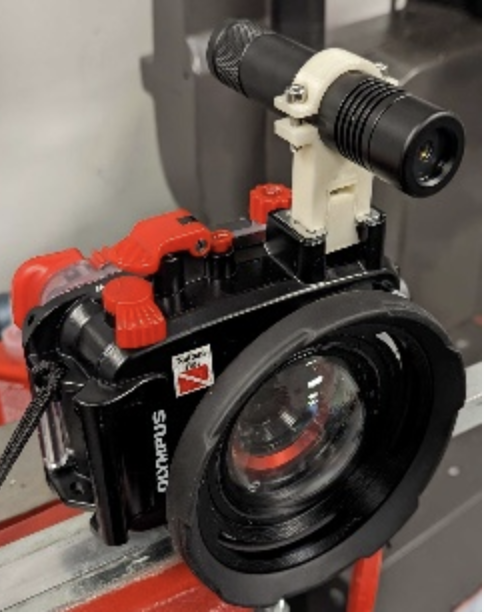
\includegraphics[width=\linewidth, keepaspectratio]{images/fishsenselite.png}
        \end{column}
        
        % Column 2
        \begin{column}{0.25\textwidth}
            \centering
            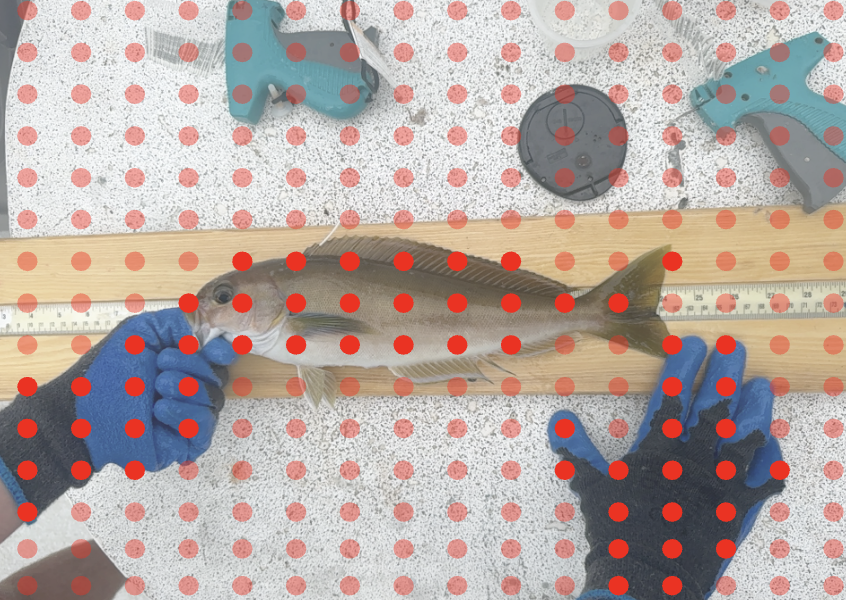
\includegraphics[width=\linewidth, keepaspectratio]{images/fish_grid_fsmobile.png}
        \end{column}
        
        % Column 3
        \begin{column}{0.25\textwidth}
            \centering
            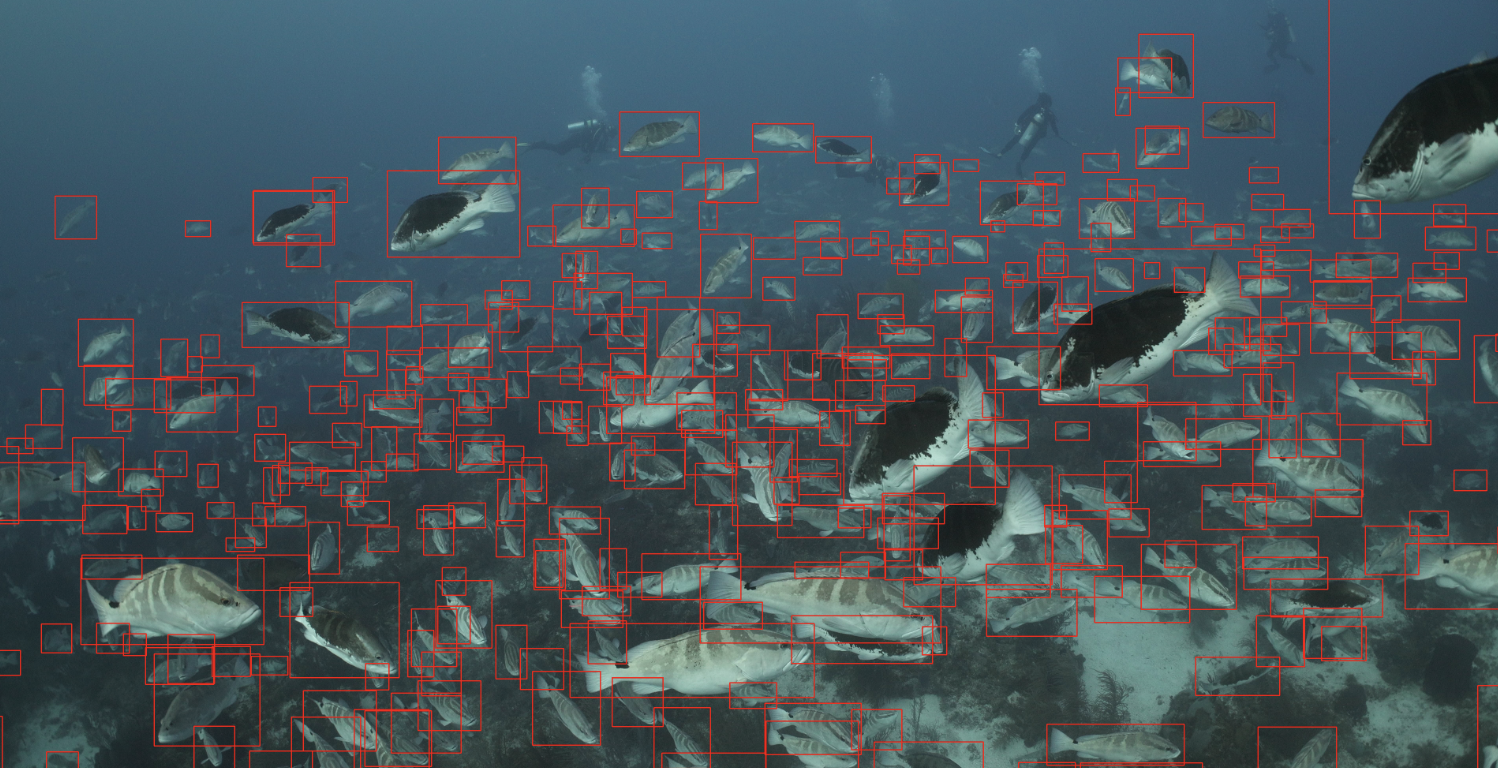
\includegraphics[width=\linewidth, keepaspectratio]{images/fishdetection.png}
        \end{column}
        
        % Column 4
        \begin{column}{0.25\textwidth}
            \centering
            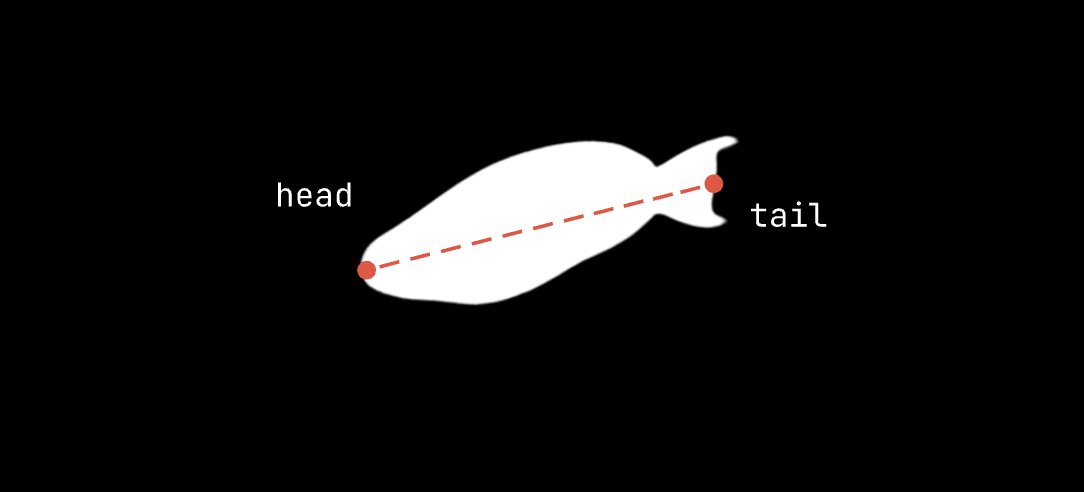
\includegraphics[width=\linewidth, keepaspectratio]{images/segmentation.png}
        \end{column}
    \end{columns}

    \begin{itemize}
        \item 3D fish imaging system to monitor fish population.
    \end{itemize}
    
    
\end{frame}

\begin{frame}
    \frametitle{Processing of Image Data}

    \centering
    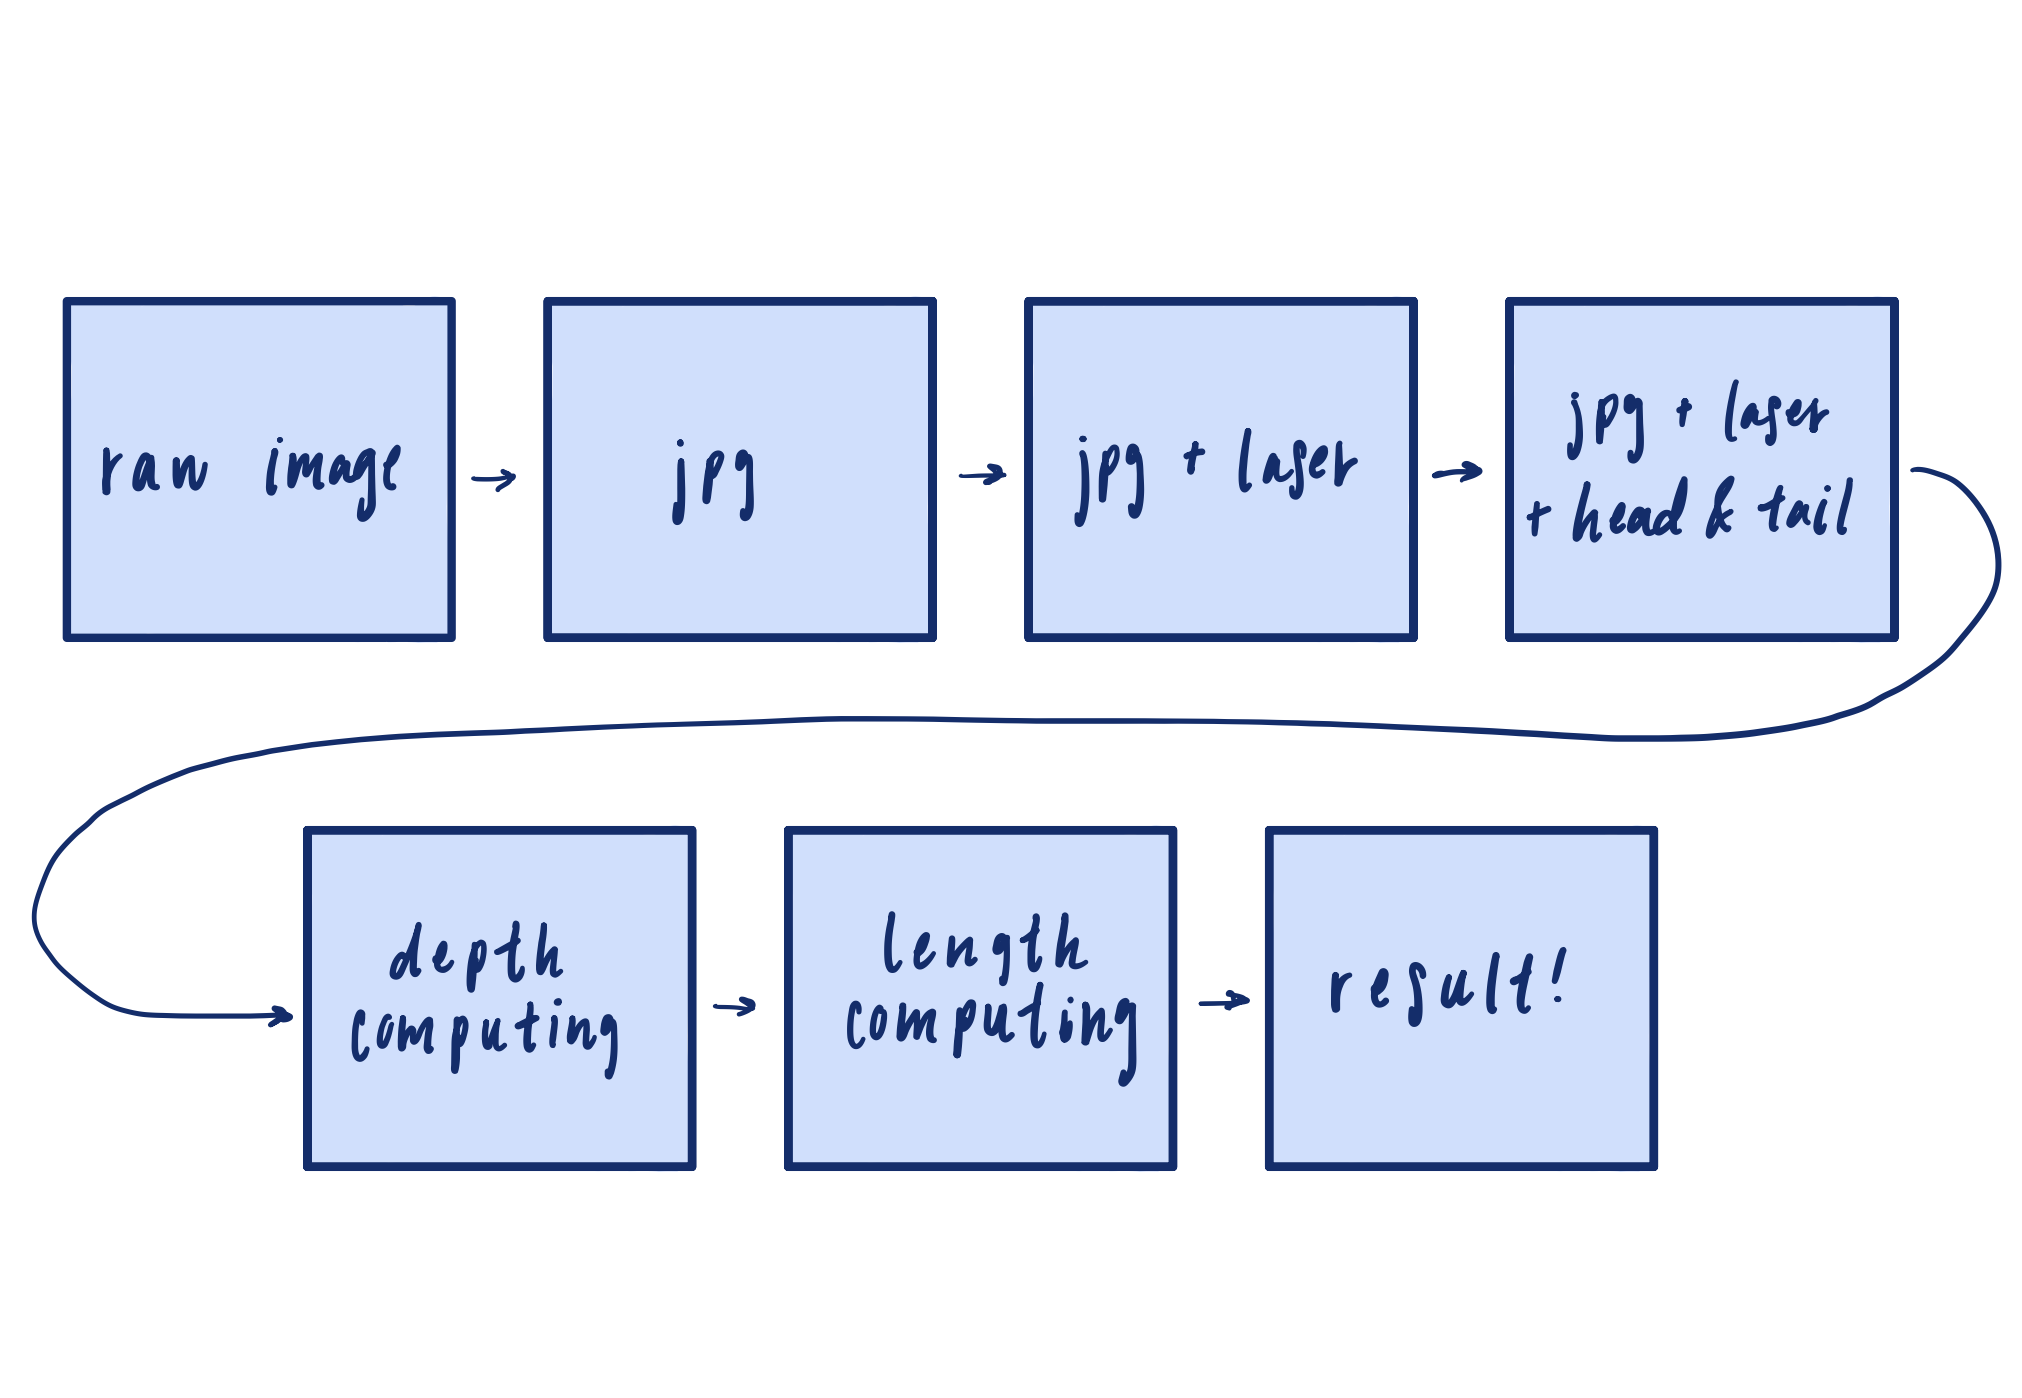
\includegraphics[width=0.8\textwidth, keepaspectratio]{images/flow1.png}
\end{frame}

\begin{frame}
    \frametitle{Processing of Image Data}

    \centering
    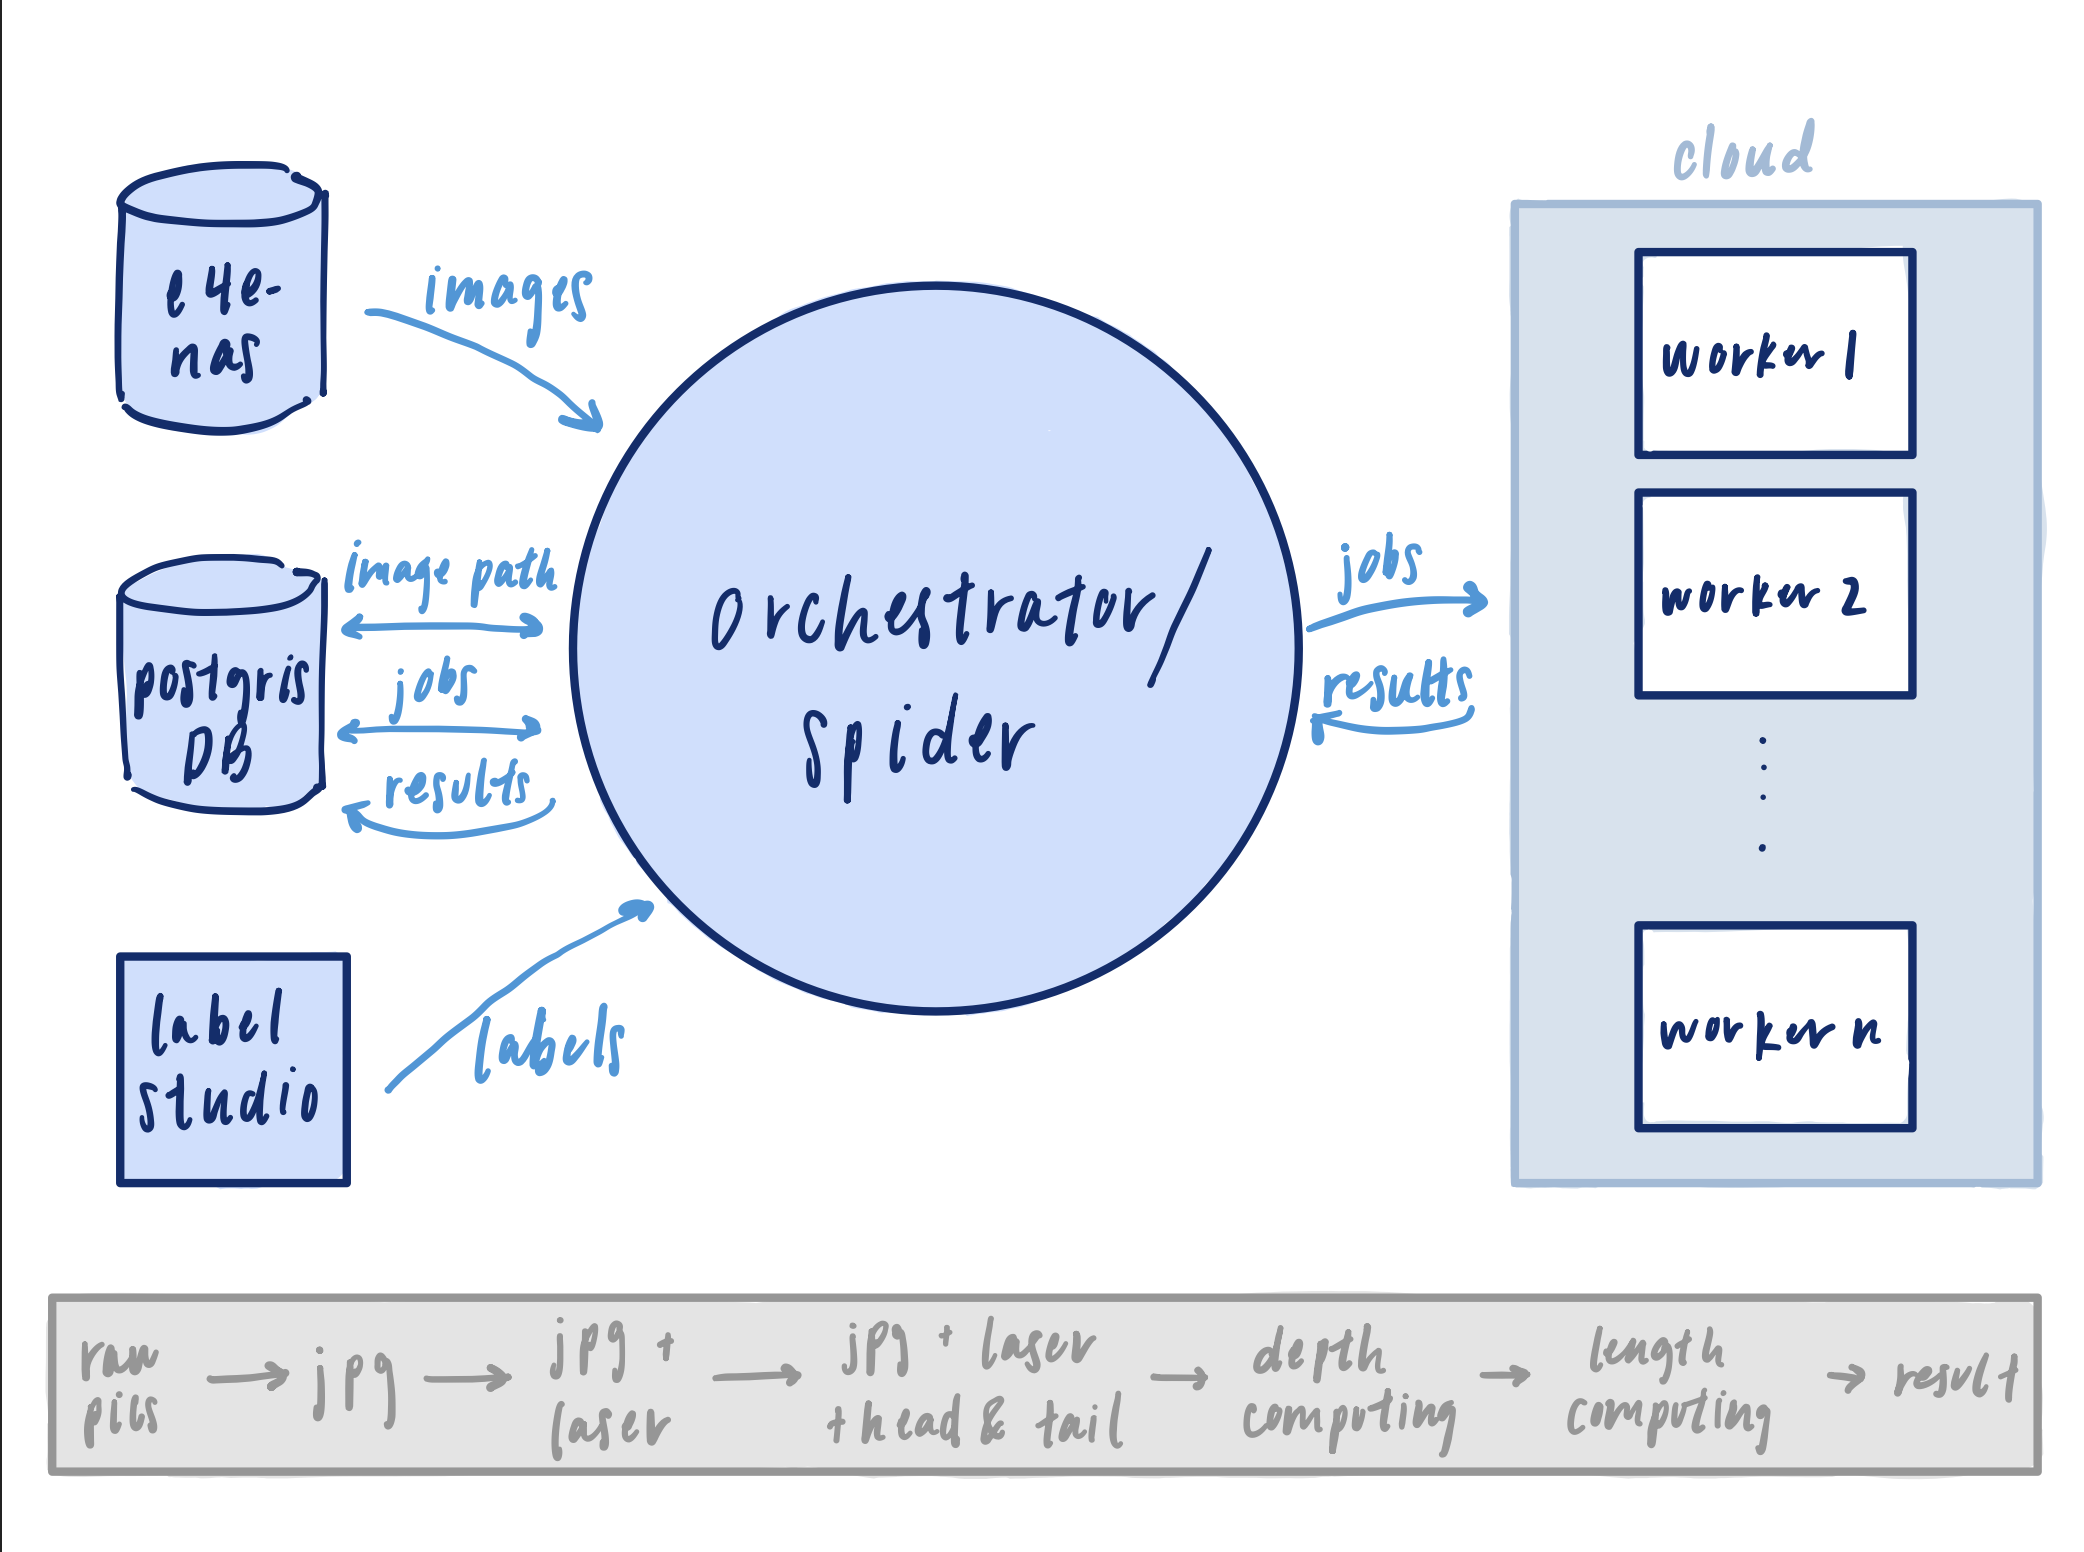
\includegraphics[width=0.8\textwidth, keepaspectratio]{images/flow2.png}
\end{frame}

\begin{frame}{Main Research Focus}
    \begin{itemize}
        \item Can Generative Adversarial Networks (GANs) improve low-light underwater images?
        \item  FishSense cameras often capture noisy, low-light images that hinder analysis.
        \item Goal: Propose and implement a GAN-based pipeline to enhance visual clarity and usable data.
    \end{itemize}
\end{frame}

\begin{frame}{Why Use GANs for FishSense?}
    \begin{itemize}
        \item FishSense images are often captured in low-light, underwater environments
        \item Traditional image processing struggles with noise and low contrast
        \item GANs are known to perform well in denoising and super-resolution tasks
        \item We aim to adapt GANs to improve underwater visual quality,
    \end{itemize}
\end{frame}

\begin{frame}{Proposed Methodology}
Based on two papers I read:
    \begin{enumerate}
        \item Region-based segmentation of underwater images
        \item Conditional GAN without random noise vector
        \item Use image superimposition: overlay multiple versions of the same scene with variations in noise, brightness, or angle
        \item Compare original vs processed image quality using SNR and visual quality metrics: SNR and Visual Quality
    \end{enumerate}
\end{frame}

\begin{frame}{Implementation Plan}
    \begin{itemize}
        \item Review relevant GAN architectures and training procedures
        \item Design and prototype in Python using PyTorch or TensorFlow
        \item Train model on collected FishSense dataset
        \item Evaluate outputs against baseline and write final paper
    \end{itemize}
\end{frame}

\begin{frame}{Additional Work: Data Collection}
    \begin{itemize}
        \item Participated in field data collection with FishSense and FishTechy
        \item Used cameras on a research boat to capture real-world training data.
    \end{itemize}
\end{frame}

\begin{frame}
    \vspace{1em}
    \centering
    \includegraphics[width=0.7\textwidth, keepaspectratio]{images/fieldop.png}
\end{frame}

% theo's slides
\begin{frame}{New Camera • Deep Water Exploration}
    \begin{columns}
        \begin{column}{0.5\textwidth}
            \centering
            \includegraphics[height=0.7\textheight,width=0.7\textwidth,keepaspectratio]{stellarHD_new_camera_image.png}
        \end{column}
        \begin{column}{0.5\textwidth}
            \begin{itemize}
            \item Test resolution in controlled water
            \item Repurpose existing materials
            \end{itemize}    
        \end{column}
    \end{columns}
\end{frame}

\begin{frame}{Underwater Optics}
    \begin{itemize}
        \item Diffractive optic. More 3D points. Depth
        \item Pinax model on more cameras (GoPro)
        \item Salinity, temp, and altitude via color and refraction
    \end{itemize}    
\end{frame}

\begin{frame}{Underwater Renderer}
    \begin{itemize}
        \item Completed: Get some HIP hardware
        \item In progress: Set up system (Specifically RedHat 9.6)
        \item Next steps: Test HIP-RT FP64 capabilities, evaluate DrJit HIP options
    \end{itemize}    
\end{frame}

\begin{frame}
    \frametitle{Vector Database}
    \begin{itemize}
        \item Our JSON database is becoming too large.
        \item Search performance is slowing down.
        \item We need a more efficient solution.
    \end{itemize}
    \vspace{0.5cm}
    \centering
    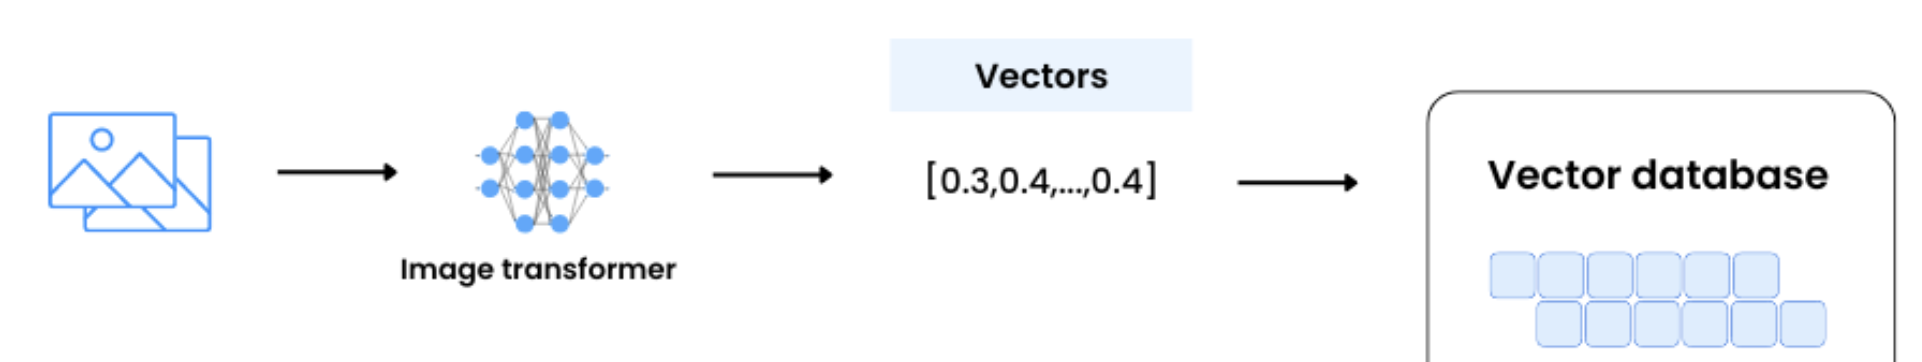
\includegraphics[width=0.8\textwidth, keepaspectratio]{images/Vectordb.png}
\end{frame}

\begin{frame}
    \frametitle{The Solution}
    \begin{itemize}
        \item Use an embedded vector database.
        \item No external server required for processing.
        \item Enables instant, efficient search results.
    \end{itemize}
\end{frame}

\begin{frame}
    \frametitle{LanceDB}
    \begin{itemize}
        \item Simple and efficient data retrieval.
        \item Fully embedded within the application.
    \end{itemize}
    \vspace{0.5cm}
    \centering
    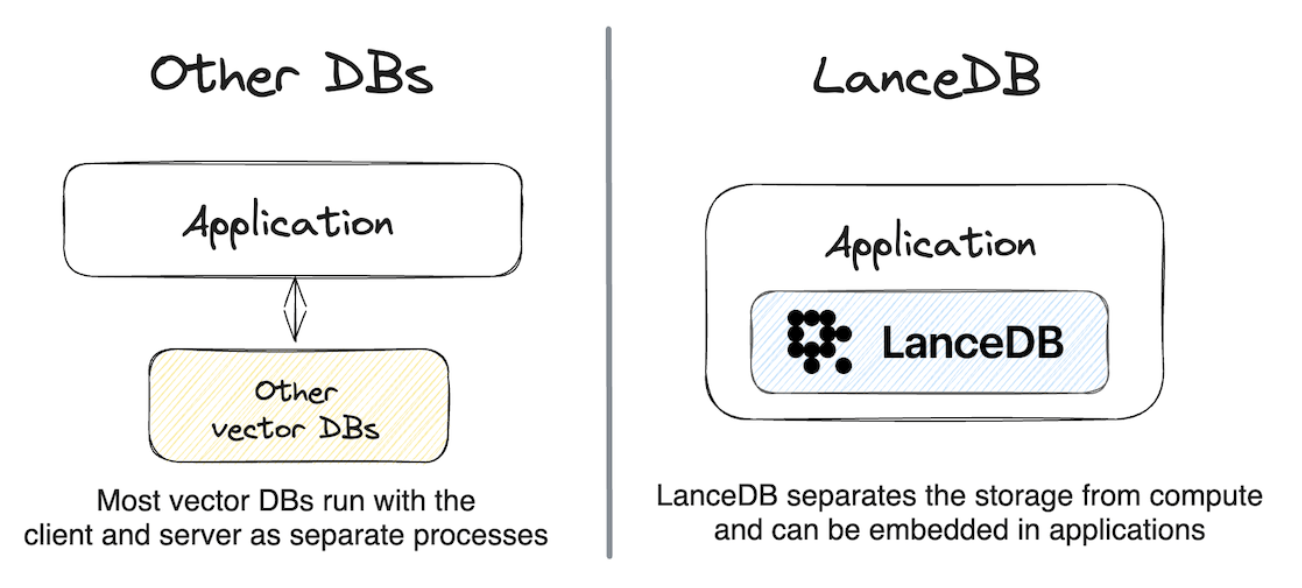
\includegraphics[width=0.8\textwidth, keepaspectratio]{images/vdbdiffernce.png}
\end{frame}

\begin{frame}
    \frametitle{Depthwise Color Constancy}
    \begin{columns}
        \begin{column}{0.5\textwidth}
            \begin{figure}
                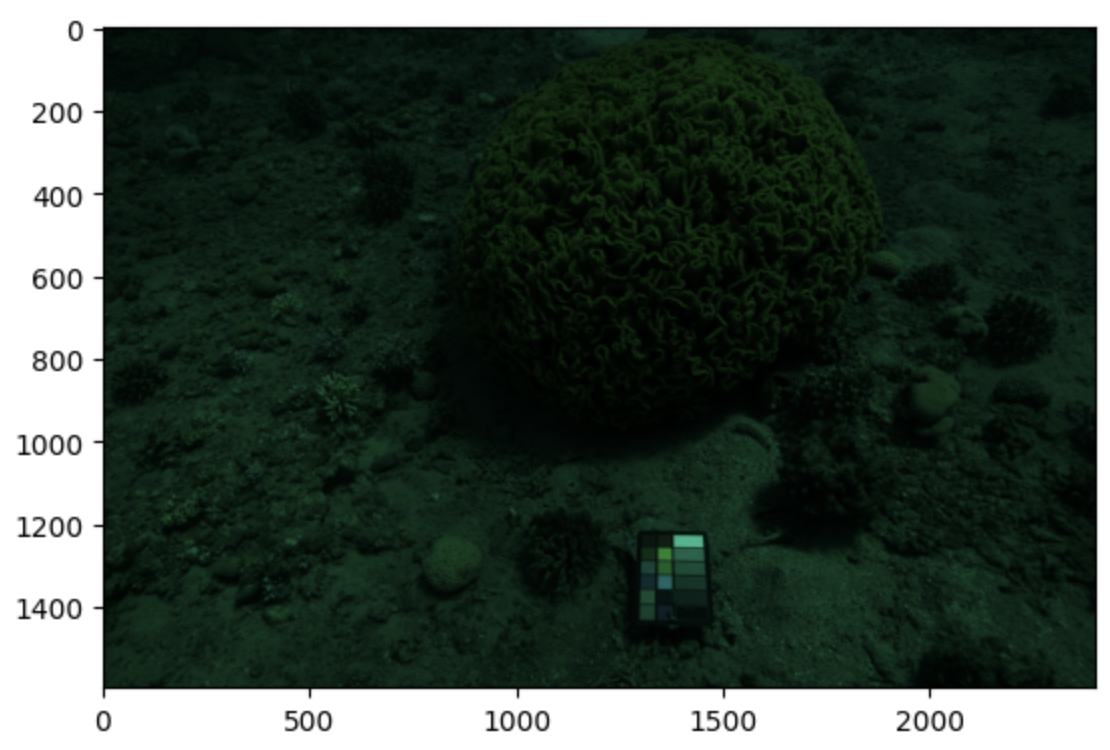
\includegraphics[width=\linewidth]{images/depth_color_issue.png}
            \end{figure}
        \end{column}    
    \end{columns}
    \begin{itemize}
        \item As depth varies, color information is lost.
        \item This makes it difficult to segment objects accurately.
        
    \end{itemize}
\end{frame}

\begin{frame}
    \frametitle{Our Solution: Depth-Aware Adaptive Convolution}
    \begin{columns}
        \begin{column}{0.4\textwidth}
            \begin{figure}
                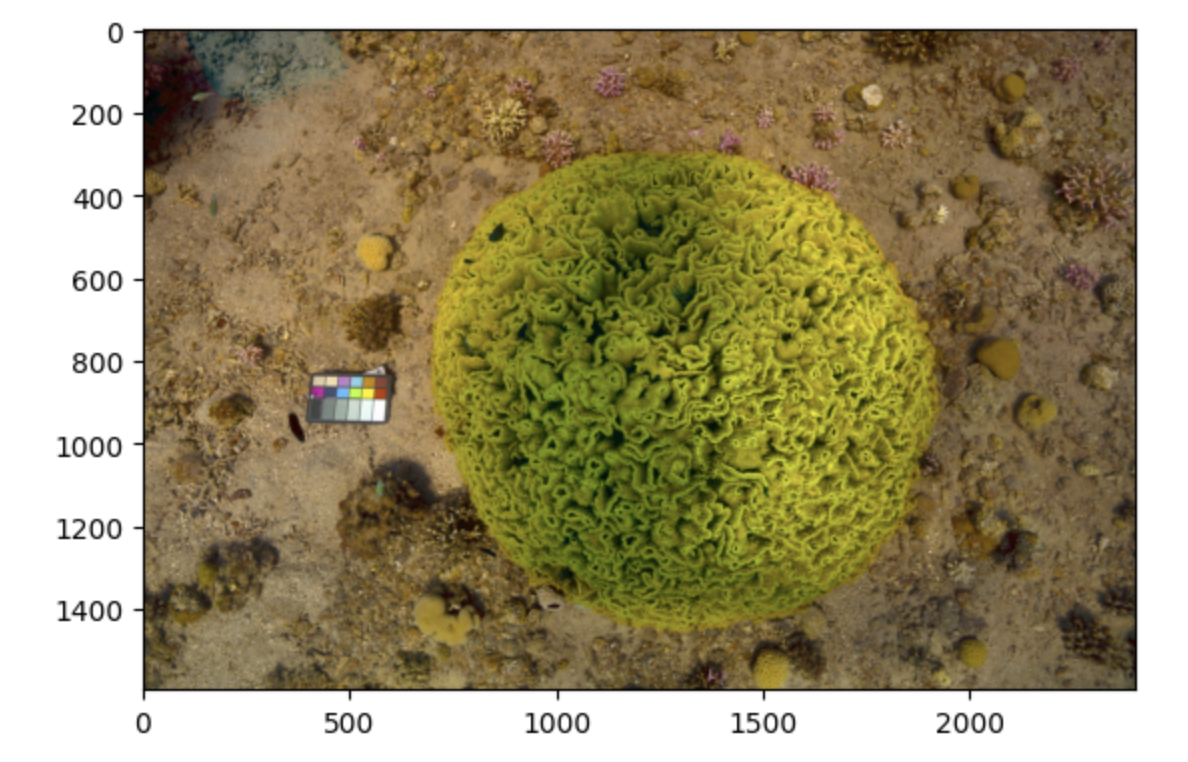
\includegraphics[width=\linewidth]{images/depth_color_corrected.png}
            \end{figure}
        \end{column}
        \begin{column}{0.6\textwidth}
            \textbf{Key Concepts:}
            \begin{itemize}
                \item Adaptive, non-fixed convolution filter.
                \item Adapts per-pixel/kernel using neighbors and depth.
                \item Enables non-uniform color correction across the image.
            \end{itemize}
        \end{column}
    \end{columns}
\end{frame}

\begin{frame}
        \frametitle{Depth-Aware Adaptive Convolution}   
    \textbf{Implementation:}
    \begin{itemize}
        \item CUDA: High-performance, parallel processing on GPUs.
        \item wgpu: Broad hardware support with Metal, Vulkan.
    \end{itemize}
\end{frame}
